\documentclass{article}
\usepackage[utf8]{inputenc}
\usepackage{hyperref}
\usepackage[letterpaper, portrait, margin=1in]{geometry}
\usepackage{enumitem}
\usepackage{amsmath}
\usepackage{booktabs}
\usepackage{graphicx}
\usepackage{amsmath}

\usepackage{hyperref}
\hypersetup{
colorlinks=true,
    linkcolor=black,
    filecolor=black,      
    urlcolor=blue,
    citecolor=black,
}
\usepackage{natbib}
\usepackage{titlesec}

\titleformat{\section}
{\normalfont\Large\bfseries}{\thesection}{1em}{}[{\titlerule[0.8pt]}]

\title{ECON7103HW2}
\author{Sedat Ors}
\date{22 January 2023}

\begin{document}

\maketitle

\section{Python}
\vspace{0.5cm}
\begin{enumerate}
\item
\noindent See Table 1 for regression results. There is significant differrence in electricity usage between two groups.
\vspace{0.5cm}
\begin{table}[]
    \centering
    \begin{tabular}{lllll}
\toprule
     &   &   Control & \multicolumn{2}{l}{Treat} \\
     &   &      Mean &      Mean & p-value \\
     &   & (Std dev) & \multicolumn{2}{l}{(Std dev)} \\
\midrule
electricity & 0 &   1181.33 &   1086.75 &    0.00 \\
     & 1 &    454.31 &    423.96 &         \\
sqft & 0 &   1633.05 &   1657.55 &    0.57 \\
     & 1 &    682.90 &    686.27 &         \\
temp & 0 &     79.89 &     79.89 &    0.99 \\
     & 1 &      2.16 &      1.97 &         \\
\bottomrule
\end{tabular}

    \caption{Regression results with heteroskedasticity-robust standard errors.}
    \label{tab:question3}
\end{table}

\item 
\noindent See Figure 1 for distribution of electricity usage for treated and control groups
\vspace{0.5cm}
\begin{figure}[]
    \centering
     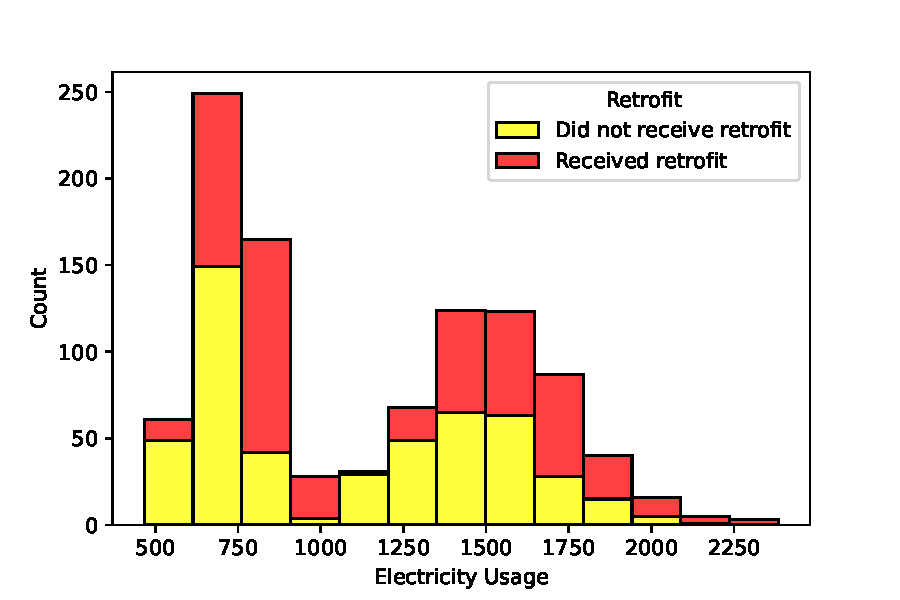
\includegraphics{histogram.pdf}
    \caption{Electricity usage}
    \label{tab:question3}
\end{figure}

\item 
\noindent See Table 2 and Table 3 for regression results
 \begin{table}[]
    \centering
    \begin{tabular}{lr}
\toprule
{} &   Estimates \\
\midrule
Constant &  -83.602758 \\
sqft     &    0.615339 \\
temp     &    3.255075 \\
retrofit & -109.666176 \\
\bottomrule
\end{tabular}

    \caption{}
    \label{tab:question3}
\end{table}

\vspace{0.5cm}
\begin{table}[]
    \centering
    \begin{tabular}{lr}
\toprule
{} &  Estimates \\
\midrule
sqft         &       0.62 \\
retrofit     &    -109.67 \\
temp         &     -83.60 \\
Observations &    1000.00 \\
\bottomrule
\end{tabular}

    \caption{}
    \label{tab:question3}
\end{table}
\end{enumerate}

\section{Stata}
\begin{enumerate}
    \item 
    
\noindent See table 4
\vspace{0.5cm}
\begin{table}[h]
    \centering
     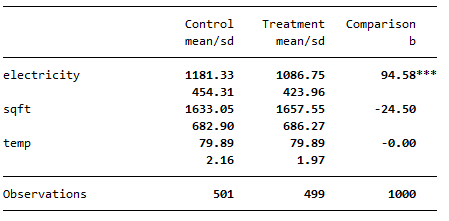
\includegraphics{HW2Q2.png}
    \caption{\(t\)-test for Treatment, Control and Difference}
    \label{tab:btable_stata}
\end{table}

\item
\noindent See table 5 
\vspace{0.5cm}
\begin{table}[]
    \centering
    \documentclass[]{article}
\setlength{\pdfpagewidth}{8.5in} \setlength{\pdfpageheight}{11in}
\begin{document}
\begin{tabular}{lc} \hline
 & (1) \\
VARIABLES & model1 \\ \hline
 &  \\
sqft & 0.615*** \\
 & (0.006) \\
retrofit & -109.666*** \\
 & (7.948) \\
temp & 3.255* \\
 & (1.924) \\
Constant & -83.603 \\
 & (154.360) \\
 &  \\
Observations & 1,000 \\
 R-squared & 0.919 \\ \hline
\multicolumn{2}{c}{ Standard errors in parentheses} \\
\multicolumn{2}{c}{ *** p$<$0.01, ** p$<$0.05, * p$<$0.1} \\
\end{tabular}
\end{document}

    \caption{Regression results with heteroskedasticity-robust standard errors.}
    \label{tab:question3}
\end{table}

\item
\noindent See figure 2 
\vspace{0.5cm}
\begin{figure}[h]
    \centering
    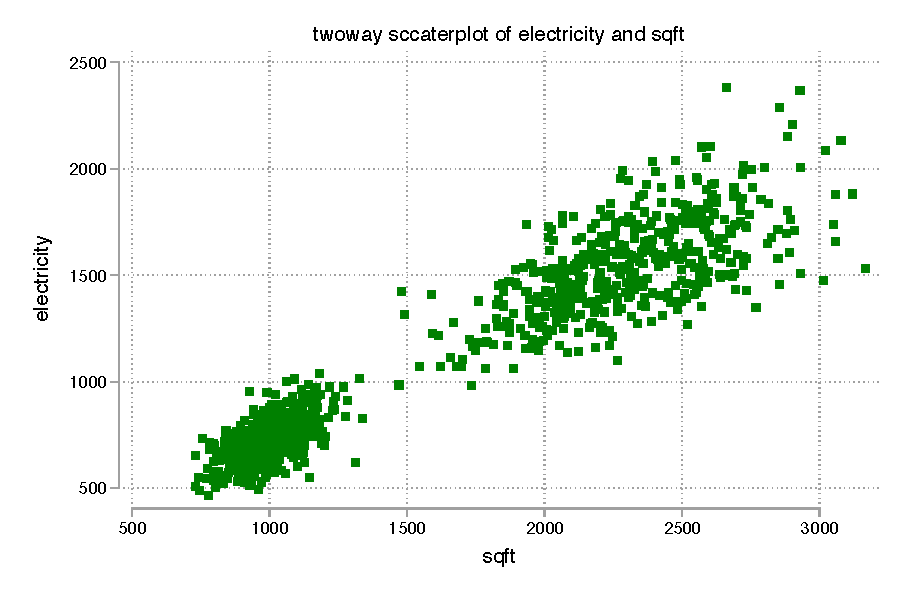
\includegraphics{HW2Q2.pdf}
    \caption{Scatterplot of electricity usage and home size}
    \label{fig:scatter}
\end{figure}
\end{enumerate}
\
\end{document}